\documentclass[10pt]{article}

\usepackage[english]{babel}
\usepackage[T1]{fontenc}
\usepackage[utf8x]{inputenc}

\usepackage{appendix}
\usepackage{amsmath}
\usepackage{cprotect}
\usepackage{listings}
\usepackage{float}
\usepackage{subcaption}
\usepackage[margin=2cm]{geometry}
\usepackage{graphicx}
\usepackage{underscore}

\lstset{
    tabsize=3,
    breakatwhitespace=true,
    breaklines=true,
    frame=simple
}

\title{Lab3 - SAT-MAX (Branch-and-Bound)}
\author{Matthew Walker - 999540475 - walker82}
\date{\today}

%1) DONETODO program flow
%   DONETODO initial "best"
%   DONETODO bounding function
%2) DONETODO plot of decision trees for all but 4
%   DONETODO counts of tree nodes visited
%   DONETODO runtime
%3) DONETODO summarize and discuss

\begin{document}

\maketitle

\section{Software Details}
\subsection{Program Flow}
\texttt{main()} is located in \texttt{sat_maxer_main.cpp} and calls \texttt{cmdargs::parse} to get the command line arguments, then calls \texttt{program_main} with those arguments. \texttt{program_main} then calls \texttt{input::parse_data} on an the file specificed by the command line options, and then calls \texttt{void branchAndBound(visitor, graph)} with a SAT-MAX visitor (\texttt{maxsat::DefaultVisitor}) and graph (\texttt{CNFTree}).

The template function \texttt{void branchAndBound(visitor, graph)}, (found in \texttt{branch_and_bound.hpp}) performs a general branch-and-bound over \texttt{graph}, calling functions on \texttt{visitor} and \texttt{graph}. \texttt{visitor} functions are called to compute costs (\texttt{evalPartialSolution}) and notify of particular events such as exploring a new vertex (\texttt{onExplore}), when leaving a subtree (\texttt{onLeave}), and when a new best solution is found (\texttt{onNewBest}). Functions on \texttt{graph} are called to get the descendants of a node (\texttt{fanout}), and to get a node's next sibling (\texttt{nextSibling}) and whether a node has any more siblings (\texttt{hasNextSibling}).

Of note is that \texttt{CNFTree} does not store anything beyond an ordering of variables -- all "vertices" are generated on the fly, and all vertex properties are derived from values stored on the vertex.

\label{sec:eval-intro}
\texttt{maxsat::DefaultVisitor} utilizes \texttt{CNFEvaluation} to compute cost on full solutions and bounds on partial solutions. \texttt{CNFEvaluation} has two modes: one "from-scratch" which uses no prior information to compute the bound function (runs in \(O(\#\text{disjunctions} \cdot \#\text{literals in disjunctions})\) time), and one "incremental" mode where where updates are applied on exploration and leave events (runs in \(O(\#\text{disjunctions that have literal that changed})\) time). The incremental mode is considerably faster, as detailed in section \ref{sec:scratch-vs-incremental}, but does not contain all attempted node-visit-count optimizations that the from-scratch mode does. Incremental mode can be enabled with \texttt{--incremental}.

\subsection{Determining an Initial Best Solution}
A simple initial solution of setting all variables to \texttt{false} was used, as all problems find a solution with the minimum cost very quickly.

\subsection{Bounding Function}\label{sec:single-unset-conflict}
The general approach used for a cost function lower bound is to determine the number of provably false disjunctions in the problem, given a (partial, or complete) setting of the variables. A simple way to do this is to loop over all the disjunctions, and to set the lower bound to the number of disjunctions where all terms are false. This what the from-scratch method does, and what the incremental method effectively does. The from-scratch method also performs a test for a simple conflict between single variables: eg. if the only unset literal in one disjunction is $!x$, and the only unset literal in another disjunction is $x$, then the number of provably false disjunctions can be incremented by one. 

\subsection{Variable Order}
Several variable orders were explored, but there is one that is much consistently better than others. The orders can be selected with the \texttt{--variable-order} option (see section \ref{sec:program-args}), and the best general ordering hierarchy (\texttt{GBD} with ties broken by \texttt{MCF}, then finally \texttt F) is set as the default. Their summaries follow:
\begin{table}[H]
\centering
\begin{tabular}{p{0.2\linewidth} | p{0.75\linewidth}}
\hline\hline
Name (\texttt{short name}) & Description \\
\hline
File (\texttt{F}) & ordered by first occurrence in the file. (complete ordering) \\\hline
Grouped by disjunction (\texttt{GBD}) & Ordered by the first disjunction that the variable appears in. (partial ordering) \\\hline
Most common first (\texttt{MCF}) & Count the total number of inverted and non-inverted occurrences of each variable, then order by most common first (usually a partial ordering) \\\hline
All but one in disjunction (\texttt{ABOID}) & Splits the variables into two groups, with the first containing most variables, and the second attempting to contain one variable from every disjunction. (partial ordering) \\\hline
\texttt{RANDOM} & completely random ordering. (complete ordering) \\
\hline
\end{tabular}
\end{table}

\section{Application}

\subsection{Performance}
\label{sec:scratch-vs-incremental}
\begin{table}[H] \centering
\begin{tabular}{r | *2{r r} | r }
\hline\hline
        & \multicolumn{2}{c|}{"from-scratch"} & \multicolumn{2}{c|}{"incremental"} \\
Problem & Nodes Visited & \multicolumn{1}{c|}{Time} & Nodes Visited & Time & max. clauses sat.\\
\hline
1.cnf & 6          &   10 ms &         14 & 7 ms & 7 \\
2.cnf & 212628     &  216 ms &     592784 & 74 ms & 79 \\
3.cnf & 88080375   &   2m 8s &   92274678 & 12.7 s & 159 \\
4.cnf & 1677721591 & 47m 46s & 1744830454 & 4m 2s & 191 \\
\hline
\end{tabular}
\caption{Nodes visited, times taken and maximum number satisfiable disjunctions for the problems}
\end{table}

\subsection{Visualizations}
\begin{figure}[H]
\centering
\subcaptionbox{\small\texttt sat-maxer -f data/1.cnf --graphics}{
	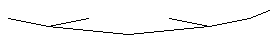
\includegraphics[width=0.45\linewidth]{assets/lab3/1.png}
}
\subcaptionbox{\small\texttt sat-maxer -f data/2.cnf --graphics}{
	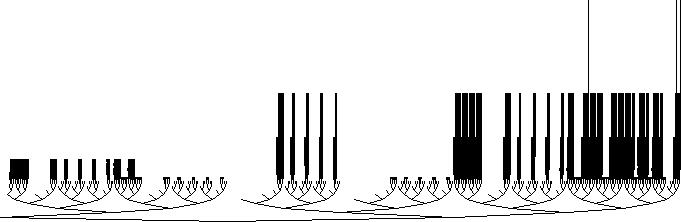
\includegraphics[width=0.45\linewidth]{assets/lab3/2.png}
}
\subcaptionbox{\small\texttt sat-maxer -f data/3.cnf --graphics}{
	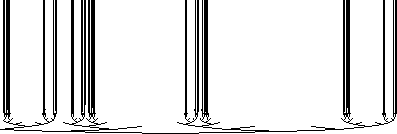
\includegraphics[width=0.45\linewidth]{assets/lab3/3.png}
}
\end{figure}

\section{Discussion}
In terms of time taken, a efficient cost computation greatly outweighs some optimizations for particular problems. The \#3 and \#4 problems seem to be extremely degenerate, and are resistant to all forms of optimization tried. All variables ocurr the same number of times both inverted and non-inverted. There seems to be some possible further node visit reductions for \#3 and \#4: scaled down versions of these problems were created (\texttt{data/3over5.cnf} and \texttt{data/3over2.cnf}) and the program was run repeatedly with \texttt{RANDOM} order, and there were many runs observed with approximately one fifth of the number of node visits. Examining these better orders led to the creation of the \texttt{ABOID} order, as that seemed to be approximately what those good runs had chosen. However, \texttt{ABOID} generally performs poorly, though \texttt{-r ABOID,GBD,RANDOM} produces a slight reduction about one-out-of-six times.

For problems of more "random" construction, such as \#2, it seems that many more optimizations can be applied. For example, the number of nodes visited with the single variable consistency check enabled (described in section \ref{sec:single-unset-conflict}) is less than half. In the more degenerate problems, this optimization only has the effect of restricting the complete solution nodes visits to 1, and partial solution node visits are unaffected.

\section*{Appendix}
\appendix
\begin{minipage}{\linewidth}
\section{Program Options}\label{sec:program-args}
\begin{lstlisting}
Program Options:
  -h [ --help ]                         print help message
  -f [ --problem-file ] arg             The file with the SAT-MAX problem to 
                                        solve
  -r [ --variable-order ] arg (=GBD,MCF,F)
                                        Comma or (single-token) space separated
                                        list of sort orders, interpreted as a 
                                        hierarchy with top level first. Valid 
                                        strings: FILE, F, GROUPED_BY_DISJUNCTIO
                                        N, GBD, MOST_COMMON_FIRST, MCF, 
                                        ALL_BUT_ONE_IN_DISJUNCTION, ABOID, 
                                        RANDOM
  --incremental                         Use incremental mode for computing 
                                        costs

Meta Options:
  --graphics                            Enable graphics
  --debug                               Turn on the most common debugging 
                                        output options
  --DL::INFO                            debug output control flag
  --DL::WARN                            debug output control flag
  --DL::ERROR                           debug output control flag
  --DL::ROUTE_D1                        debug output control flag
  --DL::ROUTE_D2                        debug output control flag
  --DL::ROUTE_D3                        debug output control flag
  --DL::PIN_BY_PIN_STEP                 debug output control flag
  --DL::MAZE_ROUTE_STEP                 debug output control flag
  --DL::ROUTE_TIME                      debug output control flag
  --DL::ROUTE_D4                        debug output control flag
  --DL::APL_D1                          debug output control flag
  --DL::APL_D2                          debug output control flag
  --DL::APL_D3                          debug output control flag
  --DL::APL_D4                          debug output control flag
  --DL::DATA_READ1                      debug output control flag
\end{lstlisting}
\end{minipage}

\end{document}
